% --------------------------------------------------------------
% This is all preamble stuff that you don't have to worry about.
% Head down to where it says "Start here"
% --------------------------------------------------------------
 
\documentclass[12pt]{article}

\usepackage{courier}
\usepackage{color}
\usepackage{listings}
\usepackage[square,numbers]{natbib}
\usepackage{tabls}
\usepackage{graphicx}
\usepackage{subcaption}
\usepackage{pdfpages}
\usepackage{mathtools}

\definecolor{dkgreen}{rgb}{0,0.6,0}
\definecolor{gray}{rgb}{0.5,0.5,0.5}




\lstset{language=python,
   basicstyle=\ttfamily,
   keywordstyle=\color{blue},
   commentstyle=\color{dkgreen},
   stringstyle=\color{red},
   numbers=left,
   numberstyle=\tiny\color{gray},
   stepnumber=1,
   numbersep=10pt,
   backgroundcolor=\color{white},
   tabsize=4,
   showspaces=false,
   showstringspaces=false}
 
\usepackage[margin=1in]{geometry} 
\usepackage{amsmath,amsthm,amssymb}
\usepackage{verbatim}
\usepackage{algpseudocode,algorithm}
\usepackage{setspace}

\newcommand{\ihat}{\ensuremath{\hat{\textbf{\i}}}}
\newcommand{\keff}{\ensuremath{k_{\mathrm{eff}}}}
\newcommand{\jhat}{\ensuremath{\hat{\textbf{\j}}}}
\newcommand{\lline}{\noindent\makebox[\linewidth]{\rule{\textwidth}{0.4pt}}}
\newcommand{\N}{\mathbb{N}}
\newcommand{\Z}{\mathbb{Z}}
\newcommand{\deriv}[2]{\frac{\mathrm{d} #1}{\mathrm{d} #2}}
\newcommand{\pderiv}[2]{\frac{\partial #1}{\partial #2}}
\newcommand{\bx}{\mathbf{X}}
\newcommand{\ba}{\mathbf{A}}
\renewcommand{\d}{\mathrm{d}}
\newcommand{\A}{\frac{(1-\alpha)}{2(1+\alpha)}}
\newcommand{\upl}{u_{\text{plane}}}
\newcommand{\upt}{u_{\text{point}}}
\newcommand{\D}{\Delta}
\newcommand{\ra}{\rightarrow}
\renewcommand{\SS}{\State}
 
\newenvironment{theorem}[2][Theorem]{\begin{trivlist}
\item[\hskip \labelsep {\bfseries #1}\hskip \labelsep {\bfseries #2.}]}{\end{trivlist}}
\newenvironment{lemma}[2][Lemma]{\begin{trivlist}
\item[\hskip \labelsep {\bfseries #1}\hskip \labelsep {\bfseries #2.}]}{\end{trivlist}}
\newenvironment{exercise}[2][Exercise]{\begin{trivlist}
\item[\hskip \labelsep {\bfseries #1}\hskip \labelsep {\bfseries #2.}]}{\end{trivlist}}
\newenvironment{problem}[2][Problem]{\begin{trivlist}
\item[\hskip \labelsep {\bfseries #1}\hskip \labelsep {\bfseries #2:}]\hspace{0.3in}\newline\newline}{\end{trivlist}}
\newenvironment{question}[2][Question]{\begin{trivlist}
\item[\hskip \labelsep {\bfseries #1}\hskip \labelsep {\bfseries #2.}]}{\end{trivlist}}
\newenvironment{corollary}[2][Corollary]{\begin{trivlist}
\item[\hskip \labelsep {\bfseries #1}\hskip \labelsep {\bfseries #2.} ]}{\end{trivlist}}
\newenvironment{problem*}[1][Problem]{\begin{trivlist}
\item[\hskip \labelsep {\bfseries #1} {\hspace{-0.2em}\bfseries:}]}{\end{trivlist}}
\newenvironment{solution}[1][Solution]{\begin{trivlist}
\item[\hskip \labelsep {\bfseries #1} {\hspace{-0.2em}\bfseries:}]\hspace{0.3in}\newline}{\end{trivlist}}
\newenvironment{solnum}[2][Solution]{\begin{trivlist}
\item[\hskip \labelsep {\bfseries #1}\hskip \labelsep {\bfseries #2:}]\hspace{0.3in}\newline\newline}{\end{trivlist}}
\newcommand{\iso}[2]{\ensuremath{^{#2}\text{#1}}}
\newcommand{\nubar}{\ensuremath{\overline{\nu}}}
 
\begin{document}
 
% --------------------------------------------------------------
%                         Start here
% --------------------------------------------------------------
 
\title{Homework 5}%replace X with the appropriate number
\author{Simon Bolding\\ %replace with your name
NUEN 629} %if necessary, replace with your course title
 
\maketitle

\clearpage

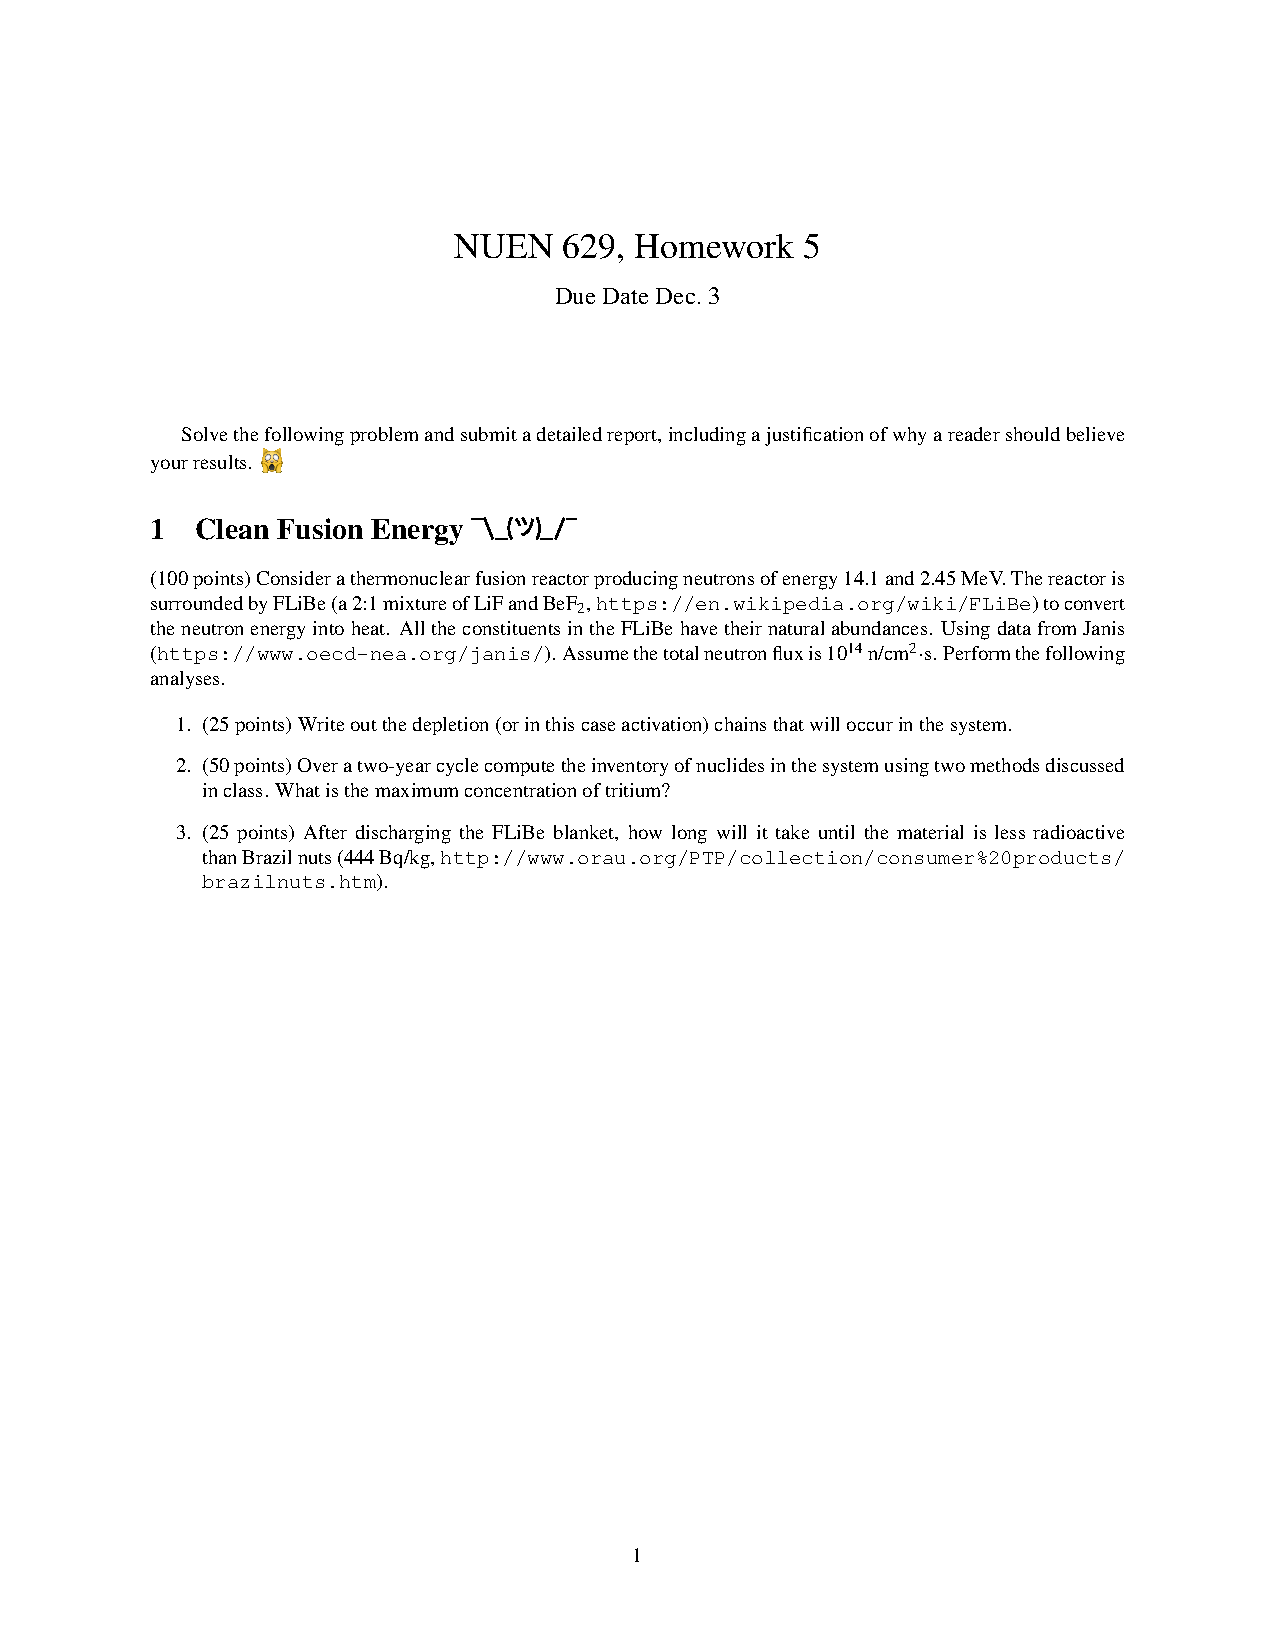
\includepdf{Homework5.pdf}

\begin{solnum}{1-1}

I tracked all of the nuclides suggested in the document \emph{FLiBE use in Fusion
Reactors: an Initial Safety Assessment} by L.C Cadwallader and G.R. Longhurst.  The decay paths from this
document are given below.  


\includepdf[pages={12,13}]{decays.pdf}

\end{solnum}
\clearpage

\begin{solnum}{1-2}

    The relative abundances of each isotope is computed assuming natural abundances and the
    chemical makeup of Li$_2$BeF$_4$.  The initial atom fractions are
    \begin{equation}
        \vec{n_0} =  \begin{pmatrix}
            ^{6}\text{Li} \\
            ^{7}\text{Li}\\ 
            ^{9} \text{Be}\\ 
            ^{19}\text{F}
        \end{pmatrix} = 
     \begin{pmatrix}
            0.0214   \\
            0.2643   \\ 
            0.1429    \\ 
            0.5714 
        \end{pmatrix} 
    \end{equation} 
    with the rest of the tracked isotopes from part 1 set to zero. 
    The neutron flux was assumed to be 90\% at 14.1 MeV and 10\% at 2.45 MeV.
    The blanket is assumed thin enough that scattering is negligible, so neutrons
    remain at these two energies, which is fairly inaccurate as Be is a strong
    moderator.
    The invetory of nuclides in the system was computed using a parabolic contour integral
    approximation to the exponential matrix and with backward Euler.  The backward Euler was implemented by taking 100 time steps
    between each data point, using the previous data point as the initial conditon.  With this approach the results were found to agree to
    with at least two digits of accuracy.  All tritium (h1) and $\alpha$ (he4)
    production are tracked as well. The plots of isotopic atom fractions are given
    below.  The mass of tritium per initial kg of FLiBe after two years of
    irradiation is computed by multiplying the atom fraction by the ratio of atomic
    masses; this ratio was found to be \boxed{1.04\times10^{-04}\text{ kg of tritium per initial kg of
    FLiBe}}.
    \begin{figure}
        \centering
        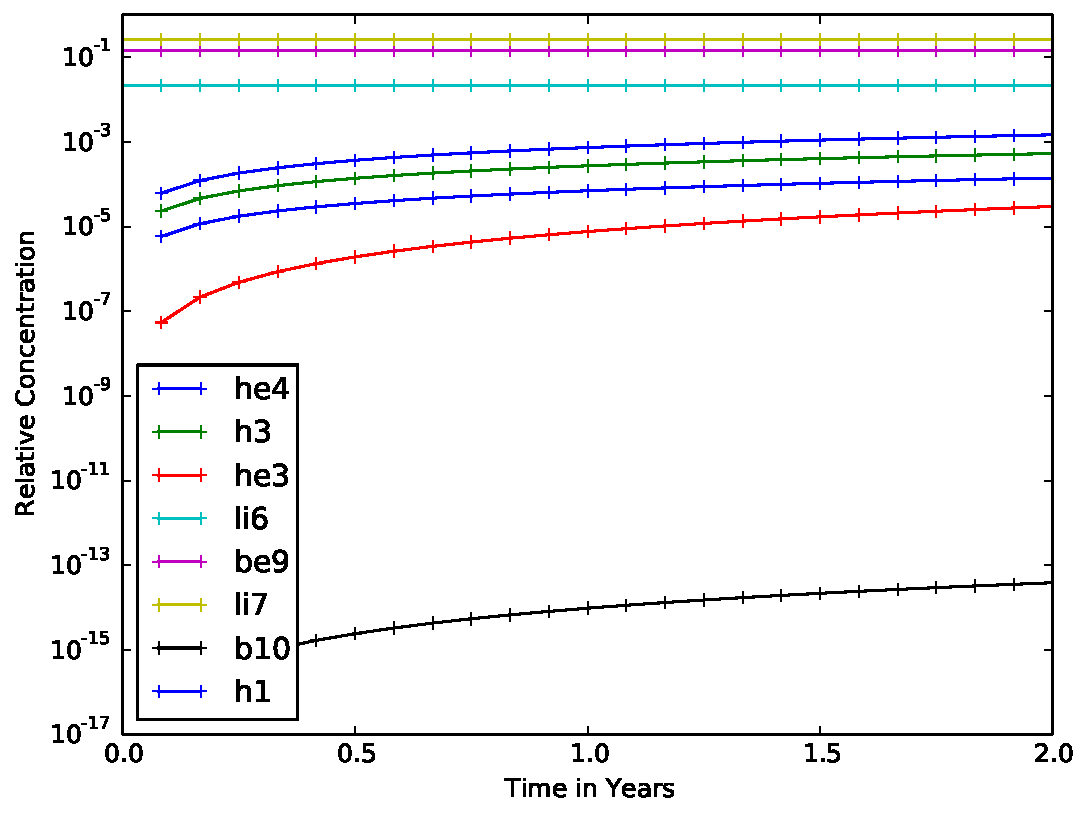
\includegraphics[width=0.5\textwidth]{p1.pdf}
    \end{figure}
    \begin{figure}
        \centering
        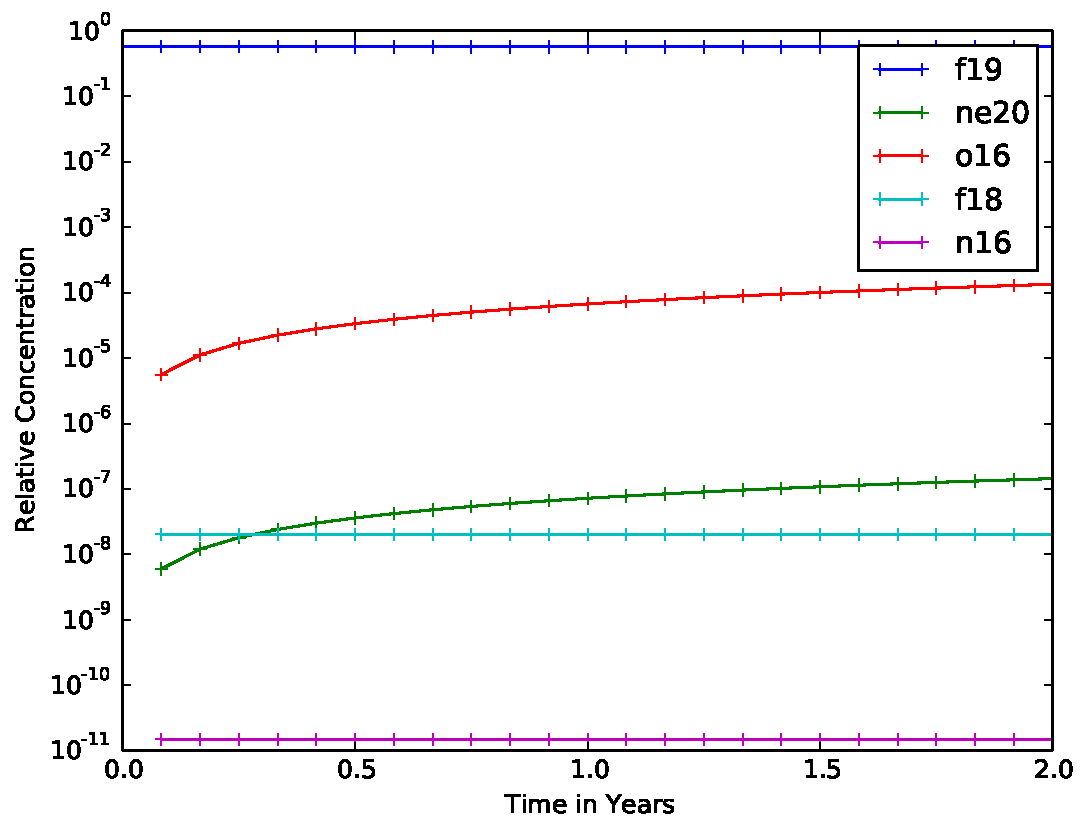
\includegraphics[width=0.5\textwidth]{p2.pdf}
    \end{figure}
    \begin{figure}
        \centering
        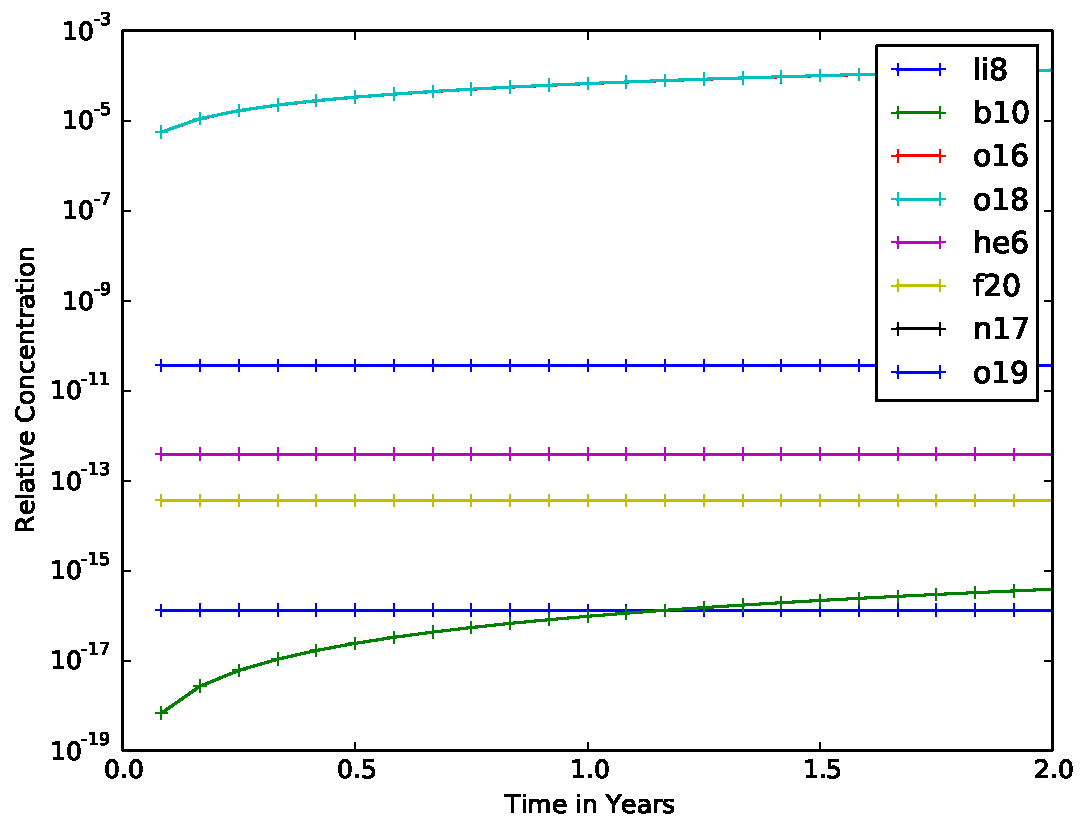
\includegraphics[width=0.5\textwidth]{p3.pdf}
    \end{figure}
\end{solnum}

\begin{solnum}{1-3}
    The activity, per unit mass of FLiBe, is computed as
    \begin{equation}
        A(t) = 7\sum_{j=1}^N \frac{\gamma_j(t)N_A}{\mathcal{A}_\text{FLiBe}}\lambda_j
    \end{equation}
    where $\gamma_j(t)$ is the atom fraction for the $j$-th of $N$ isotopes at time
    $t$ after irradiation stops. The matrix
    exponential and backward Euler were found to be numerically inaccurate for computing the new
    activities of isotopes, resulting in negative answers, due to the large range of
    decay constants relative to the time scale.  Instead, the
    atom fractions were computed ignoring secondary decay chains as
    \begin{equation}
        \gamma_j(t) = \gamma_j(t_0)e^{-\lambda_j t}
    \end{equation}
    where $\gamma_j(t_0)$ is the atom fractions after irradiation stops at 2 years.
    The factor of 7 is because my atom fractions are normalized to be atom of isotope
    $j$ per any atom in the system, rather than per mol (which would not sum to 1).  With this
    approach, it was found it will take \boxed{395\times 10^3\text{ years}} before the activity is below the threshold of 444 Bq/kg.
    This is completely dominated by the slow decay of $^{10}$Be, although the
    majority of the radioactivity is removed within 100 years once the tritium has
    decayed away.
\end{solnum}

\clearpage
\subsubsection*{Code}
\lstinputlisting[basicstyle=\scriptsize]{exp.py}

\end{document}

